\documentclass[titlepage,11pt,a4paper]{article}

\usepackage[T1]{fontenc}
\usepackage[utf8]{inputenc}
\usepackage{lmodern}
\usepackage[french]{babel}
\usepackage{url,csquotes}
\usepackage[hidelinks,hyperfootnotes=false]{hyperref}
\usepackage[titlepage,fancysections]{polytechnique}
\usepackage{amsmath}
\usepackage{amssymb}
\usepackage{mathrsfs}
\usepackage{wrapfig}
\usepackage{graphicx}
\usepackage{multicol}
\usepackage{stmaryrd}
\usepackage{textcomp} %permet de faire le °
\usepackage{algorithm}
\usepackage{algorithmic}
\usepackage{listings} %permet d'inclure du java

%Ajouter ça pour le code en couleur :

\lstset{
language=php,
basicstyle=\normalsize, % ou ça==> basicstyle=\scriptsize,
upquote=true,
aboveskip={1.5\baselineskip},
columns=fullflexible,
showstringspaces=false,
extendedchars=true,
breaklines=true,
showtabs=false,
showspaces=false,
showstringspaces=false,
identifierstyle=\ttfamily,
keywordstyle=\color[rgb]{0,0,1},
commentstyle=\color[rgb]{0.133,0.545,0.133},
stringstyle=\color[rgb]{0.627,0.126,0.941},
numbers=left,
}


\title{Fourbix}
\logo{../images/logo/accueil-logo.png}
\subtitle{INF473W Modal Web - Rapport de projet}
\author{Alexandre \bsc{Binninger} - Gabriel \bsc{Oliveira Martins}}
\date{\today}

\begin{document}

\maketitle

\clearpage

\setcounter{page}{1}


\section{Utilisation du site}

\subsection{A quoi sert ce site ?}

\emph{FourbiX} est un site de prêt de matériel par les binets. Il permet ainsi aux utilisateurs de consulter les offres des binets et de réaliser facilement leur demande en ligne. L'échange entre les binets est alors facilité et les démarches sont fluidifiées. Le nom du site est inspiré du mot d'argot militaire <<fourbi>> qui désigne l'ensemble des possessions d'un soldat.

Nous avons travaillé avec GitHub pour gérer ce projet et vous pouvez trouver le dépôt à l'adresse suivante : \url{https://github.com/gabrieloliveiragom/fourbix}. 


\subsection{Comment utiliser FourbiX ?}

Sur \emph{FourbiX}, plusieurs possibilités s'offrent à l'utilisateur pour effectuer ses recherche. Il est par exemple possible de taper directement le nom d'un item dans la barre de recherche ou alors de rechercher un binet dans le catalogue. Les pages des binets exposent le matériel qu'ils mettent à disposition et il suffit de cliquer sur un objet pour arriver sur sa page dédiée et ainsi réaliser une demande. Les demandes peuvent être faites à son propre nom ou au nom d'un binet auquel on appartient. On peut les consulter directement via la page dédiée "Demandes".\\

Certaines informations sur l'objet sont disponibles : évidemment son nom et la quantité restante, mais il est possible pour un responsable matériel du binet d'indiquer une courte description et de déposer une photo de l'objet qui seront affichées dans le caroussel du catalogue. Le binet peut fixer une caution s'il le souhaite.\\

Les Administrateurs de binet peuvent gérer les membres dudit binet. Les responsables de matériel gèrent le matériel et les demandes associées. Ceux qui sont simplement "membres" du binet peuvent faire une demande au nom de ce binet. Pour être administrateur du site, il faut être administrateur du binet "Administrateurs" et il est alors possible de gérer tous les binets, de rajouter des binets et des utilisateurs et d'en supprimer.\\

Lorsqu'un utilisateur fait une demande à un binet, les responsables matériel de ce binet peuvent alors accepter la demande sur la page. Une deadline est renseignée, date à partir de laquelle le binet se donne le droit d'encaisser une caution éventuelle. Toutes les demandes qui donnent cours à un prêt sont stockées, il sera donc toujours possible de consulter la BDD en cas de contentieux.

\subsection{Gestion du matériel et du personnel}

La page des binets permet de gérer le matériel : possibilité d'ajouter un nouvel item ou de modifier les caractéristiques d'un item déjà présent. Il est possible de le faire directement sur le tableau. Bien sûr, ces options de modification n'apparaissent pas pour un utilisateur normal pour lequel l'affichage est alors un peu moins lourd.\\

Un utilisateur ne peut pas demander via le site à rejoindre un binet. C'est à un administrateur du binet ou du site de le rajouter manuellement via le panneau correspondant. La liste des personnes appartenant au binet, ainsi que leur rôle, est affiché sur la page du binet sur un leaderboard.

\section{Le Front-end}

\subsection{HTML5/CSS3}

\subsubsection{Aspect du site}

\begin{wrapfigure}[8]{r}{4cm}
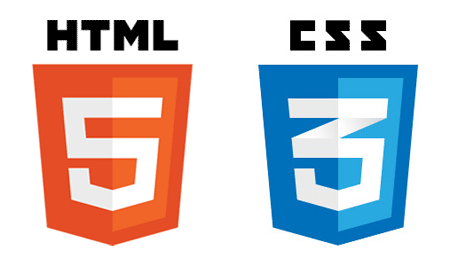
\includegraphics[scale=0.3]{html5-css3.png}
\end{wrapfigure}
Les langages HTML5 et CSS3 permettent de mettre en forme le site. Chaque page de notre site web commence par un \emph{jumbotron} qui affiche le nom de la page, une courte description de son contenu et une image représentative. Pour la page des binets, l'image affichée est le logo du binet s'il a été renseigné ou une image par défaut sinon. Les items possèdent également une image par défaut.\\

Notre affichage possède plusieurs points de personnalisation important. Premièrement, nous avons utilisé une police non standard pour afficher à plusieurs reprises le nom de notre site web. L'importation d'une police personnalisée est réalisée via l'instruction \emph{@font-face} de CSS. Pour le Background, que nous avons souhaité sobre, nous utilisons la balise <body> et nous répétons un pattern coloré. En revanche, le background des classes .container (de Bootstrap) est fixé sur la couleur blanche : cela permet de créer un contraste entre les espaces du site web où se situe l'information et ceux qui n'en possèdent pas.\\

L'utilisation de Bootstrap nous a permis de rendre notre site un minimum responsive design. Bien que nous n'ayons pas centré tout notre effort de développement sur cet aspect, il n'a pas été négligé et nous avons tenu à ce que l'affichage reste correct sur des écrans de taille moyenne.

\subsubsection{Utilisation de Bootstrap}

\begin{wrapfigure}[8]{l}{4cm}

\includegraphics[scale=0.12]{bootstrap.png}
\end{wrapfigure}
Bootstrap nous a été fortement utile, notamment pour la disposition de nos différents éléments et la mise en forme qui accompagne les classes qu'il propose. Nous l'utilisons pour mettre en place nos panneaux avec un style homogène, pour l'affichage de nos tableaux (\textbf{qui sont triables}), pour la mise en place de nos formulaires, pour rajouter des <<glyphicon>>, pour afficher un \emph{jumbotron} au début de chaque page, pour afficher la barre de navigation.\\

Un des autres points forts de Bootstrap a été la mise en place du caroussel. Bootstrap propose pour cela des classes qui sont personnalisables avec le CSS (par exemples les boutons de défilement). Il faut notamment faire attention à toujours définir une slide "active" qui sera affichée en premier.\\


\subsection{Javascript et JQuery}

Javascript est ce qui permet de rendre le site dynamique. Des aspects de Javascript sont déjà utilisés implicitement par Bootstrap, par exemple avec le défilement du caroussel.\\

\begin{center}

\includegraphics[scale=0.25]{js-jquery.png}
\end{center}

Une fonctionnalité que nous avons implémenté en Javascript a été le cas classique de cours : alterner entre l'affichage et la dissimulation de contenu (avec \emph{slideToggle}). Dans notre cas, nous voulions afficher le contenu d'un panneau en cliquant sur le \emph{heading}. La difficulté a été de trouver le selecteur correct pour éviter de devoir définir une classe différente à chaque nouveau panneau. Nous avons pour cela décider de procéder comme suit : le \emph{heading} du panneau reçoit la classe \emph{isClickable}. Lorsque nous cliquons sur cette classe, nous devons faire appel au panneau entier de classe \emph{toBeClicked} et afficher le panel body correspondant de classe \emph{toBeToggled}. Le selecteur revient alors à prendre l'enfant du parent de ce qui est cliquable, c'est à dire : 

\begin{lstlisting}[title=Affichage des éléments dans un panneau]
$('.toBeToggled').hide();
$('.isClickable').click(function(){
   $(this).parent('.toBeClicked').children('.toBeToggled').slideToggle("slow");
   });
\end{lstlisting}


\section{Le Back-end}

\subsection{La Base de Données}

Cette section explique la manière dont la base de données a été conçues. La BDD \emph{FourbiX} est constituée des tables \textbf{\emph{utilisateurs}} et \textbf{\emph{binets}} reliés par une table relationnelle \textbf{\emph{membres}} qui relie chaque utilisateur à leur \textbf{\emph{role}} dans le binet correspondant. Les informations des \textbf{\emph{items}} sont reliées à un binet en particulier. Ils sont notamment d'un certain type (dans \textbf{\emph{types}}). Les utilisateurs peuvent réaliser pour chaque item des \textbf{\emph{demandes}} qui peuvent être acceptées : elles deviennent alors des \textbf{\emph{pretoperation}}s qui seront archivées dans la BDD si l'objet est rendu ou dont la \textbf{\emph{caution}} sera encaissée dans le cas contraire. L'utilisateur peut remonter des bugs (\textbf{\emph{bugreports}}) à l'équipe d'administration du site.\\

\begin{center}
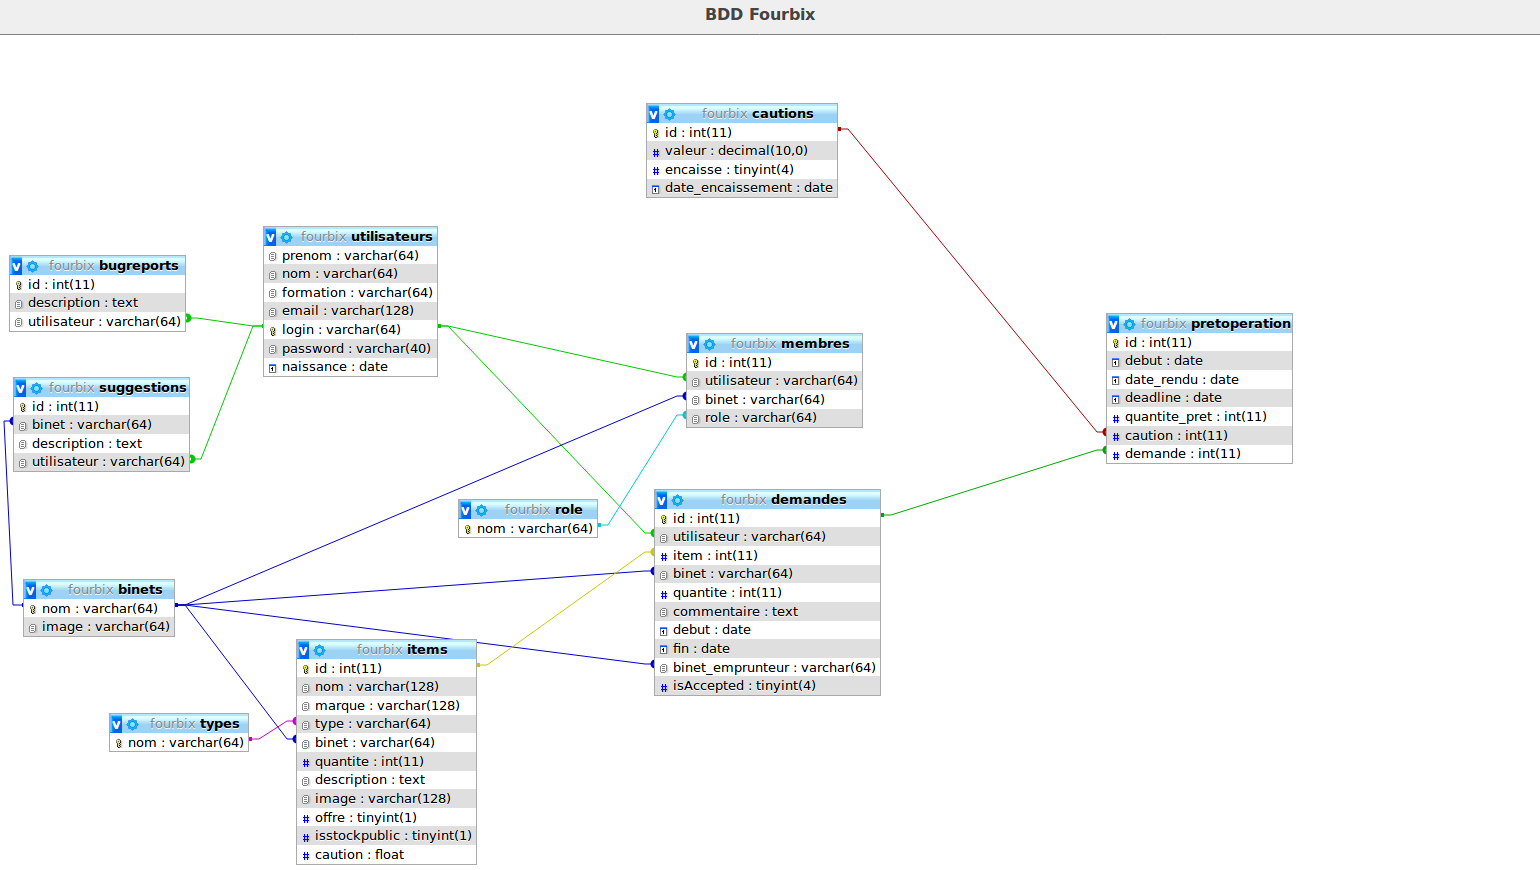
\includegraphics[scale=0.3]{BDD_FourbiX.png}
\end{center}

Toutes les tables sont reliées entre elles par des clefs étrangères lorsque cela est nécessaire. La suppression d'entrées est ajustée pour que les données soient correctement mises à jour. Par exemple, supprimer un binet ou un utilisateur supprime son entrée dans \textbf{\emph{membres}}, mais supprimer un élément de \textbf{\emph{membres}} ne supprime pas le binet ni l'utilisateur.

\subsection{Le traitement en PHP}

\begin{center}

\includegraphics[scale=0.05]{php.png}
\end{center}

Nous utilisons PHP pour gérer l'utilisation de la base de données ainsi que des éléments de sécurité

\subsubsection{Requêtes SQL}

Nous allons ici exposer quelques détails sur les requêtes SQL intéressantes. Nous parlerons également des difficultés que nous avons eues et des solutions que nous avons apportées.\\

La première requête SQL délicate fut celle de la barre de recherche. En effet, il semble peu probable qu'un utilisateur connaisse parfaitement le nom de l'item qu'il cherche à acquérir. Nous avons pour cela utilisé l'instruction conditionelle \emph{LIKE CONCAT('\%', :search, '\%')} qui permet de tester si la chaîne recherchée est une sous-chaîne du nom de l'item ou de sa marque.\\

Lorsque nous affichons sur la page des binets le \emph{leaderboard}, nous avons souhaité que les noms n'apparaissent qu'une fois. Pour cela, nous avons essayé de ruser avec la syntaxe de SQL. Nous initialisons une variable $\$userQueue="''"$ que nous remplissons à chaque nouvel utilisateur avec l'instruction $\$userQueue=\$userQueue.", '\$login'";$. Nous pouvons alors utiliser dans la requête SQL sur les utilisateurs l'instruction \emph{`utilisateur` NOT IN (\$userQueue)}. Le problème d'une telle méthode, c'est qu'elle n'est pas sécurisée et qu'une injection SQL est possible. Nous avons donc utilisé une autre méthode : nous instancions pour \$userQueue un tableau et nous récupérons tous les login dans la requête SQL : c'est ensuite php qui va tester si notre login a déjà été utilisé, et si ce n'est pas le cas, nous mettons à jour la variable \$userQueue.\\

Nous proposons sur notre site un système d'upload d'image. Nous nous sommes rendus compte qu'il n'était pas possible d'inclure directement dans la BDD le fichier image, nous avons alors procédé en insérant dans la BDD le nom de l'image à afficher. L'upload d'une image se fait en utilisant la variable globale \emph{\$\_FILE}. Cette variable va en effet stocker toutes les informations nécessaires à l'upload d'un fichier : son nom et son son poid par exemple (l'aspect sécuritaire sera détaillé à la prochaine partie). Lorsque les tests de sécurité sont effectué, nous devons renommer l'image : en effet, il se pourrait que deux utilisateurs téléversent deux images différentes avec le même nom, ce qui génèrerait des conflits. Pour éviter cela, nous renommons l'image des items en utilisant le format \emph{"image".\$nomItem.\$date('YmdHis').".png"} : à moins que deux utilisateurs téléversent une image pour deux items avec le même nom au même moment à la seconde près, nous avons la garantie de l'unicité du nom de l'image. Pour les binets, nous utilisons simplement le nom du binet qui est une clef primaire pour renommer l'image.\\

Enfin, nous utilisons la caractéristique selon laquelle \emph{\$sth->execute()} renvoie un booléen en fonction de la réussite du traitement de la demande. Cela nous permet d'afficher à l'écran un message de confirmation lorsque les opérations sur la base de données sont un succès.



\subsubsection{La sécurité}

Comme PHP est le langage qui traite les données du côté du serveur, c'est en PHP que nous gérons l'aspect sécuritaire de notre site web. Cela passe notamment par l'utilisation de PDO et des instructions \emph{\$sth=\$dbh->prepare()} et \emph{\$sth->execute(array('valeur 1', 'valeur 2'...))} vues en cours, ainsi que l'utilisation de \emph{htmlspecialchars}. Nous utilisons php pour vérifier qu'un utilisateur est loggué via les variables de session. La page Administration, par exemple, n'est accessible que si l'utilisateur est bien un administrateur. Ainsi, il ne suffirait pas à un utilisateur malveillant de rentrer dans la barre d'adresse \emph{page=administration} pour accéder au tableau d'administration du site. Un autre point de sécurité sensible est l'importation de fichier. Il nous a fallu vérifier d'une part que le fichier était d'une extension raisonnable (pour une image : jpeg, jpg, png ou gif) pour éviter qu'un utilisateur malveillant importe un script ou un fichier php susceptible d'être lu par le serveur, d'autre part que le poids du fichier était raisonnable en fixant une limite à 1Mo (ce qui est largement suffisant pour une photo le plus souvent indicative). Pour cela, nous avons utilisé la variable globale \emph{\$\_FILE} avec le code suivant :

\begin{lstlisting}[title=Securite upload image]
if (isset($_FILES['imageItem']) && $_FILES['imageItem']['name']!=""){
            if ($_FILES['imageItem']['error'] > 0){
            switch($_FILES['imageItem']['error']){
                case 4 : //"UPLOAD_ERR_NO_FILE"
                    $error_file="L'image n'a pas ete televersee.";
                    break;
                case 1 : //"UPLOAD_ERR_INI_SIZE"
                    $error_file="L'image est trop grosse !";
                    break;
                case 2 : //"UPLOAD_ERR_FORM_SIZE"
                    $error_file="L'image est trop grosse !";
                    break;
                case 3 : //"UPLOAD_ERR_PARTIAL"
                     $error_file="L'image n'a pas ete completement televersee.";
                    break;
                default :
                    $error_file="ERREUR";
                    break;
            }
        } else{
            if ($_FILES["imageItem"]['size']>1048576){ $error_file="L'image est trop grosse !";}
            $extensions_valides = array( 'jpg' , 'jpeg' , 'gif' , 'png' );
            $extension_upload = strtolower(  substr(  strrchr($_FILES['imageItem']['name'], '.')  ,1)  );
            if (!in_array($extension_upload,$extensions_valides) ){ $error_file="Extension incorrecte ($extension_upload).";}
        }
        
        if (isset($error_file)){
           echo "<div><span class='enregistrement-invalide'>Upload impossible : $error_file</span></div><br/>"; //erreur rencontree : il faut avoir tous les droits sur le dossier /image
        } else{
        ...
        }
\end{lstlisting}

Le traitement des caractéristiques de l'image est bien réalisé côté serveur et les modifications par un utilisateur malveillant de l'HTML ne devrait pas permettre d'outrepasser les limites fixées.

\section{Conclusion}

Le Modal Web a été une expérience enrichissante et la réalisation de FourbiX aura eu le double avantage de nous permettre de réaliser un projet concret en informatique et de proposer un service qui saura trouver une utilité auprès des élèves de l'École Polytechnique.

\end{document}